\lab{Algorithms}{Conditioning and Stability}{Conditioning and Stability}
\objective{Explore the condition of problems and the stability of algorithms.}
\label{lab:conditioning_stability}


\begin{equation*}
\mathlarger{ \mathlarger{ \mathlarger{f:X \rightarrow Y}}}
\end{equation*}
\begin{center} vs. \end{center}
\begin{equation*}
\mathlarger{ \mathlarger{ \mathlarger{\hat{f}:\hat{X} \rightarrow \hat{Y}}}}
\end{equation*}

%\begin{eqnarray}
%\mathlarger{\mathlarger{\mathlarger{f:X \rightarrow Y}}}\\ \mathlarger{\mathlarger{\mathlarger{ f:\hat{X} \rightarrow \hat{Y} }}}\\
%\mathlarger{\mathlarger{\mathlarger{ \hat{f}:X \rightarrow Y }}}%\\
%%\mathlarger{\mathlarger{\mathlarger{ \hat{f}:\hat{X} \rightarrow \hat{Y} }}}
% \end{eqnarray}
% 

\section*{Conditioning of a Problem}

%\begin{equation*}
%\mathlarger{ \mathlarger{ \mathlarger{f:\hat{X} \rightarrow \hat{Y}}}}
%\end{equation*}

A \emph{problem} is a function $f:X \rightarrow Y$, where $X$ is a vector space of data and $Y$ is a vector space of solutions. In a perfect world, this function takes an exact input $x$ and correctly returns the exact answer $y$. However we are working in the finite world of computers.

Since $X$ and $Y$ are vector spaces of infinite cardinality, we cannot represent these spaces on a computer perfectly. We can only represent finite subsets $\tilde{X} \subset X$ and $\tilde{Y} \subset Y$. This means that the best we can do is approximate $x \in X$ with some $\tilde{x} \in \tilde{X}$ and return an approximate correct answer $\tilde{y} \in \tilde{Y}$. But if we change the input from $x$ to $\tilde{x}$, how much will our output change?

We define the \emph{condition number} of $f$ at $x$. Let $\delta x$ denote a small perturbation of $x$, and let $\delta f = f(x+\delta x) - f(x)$. Then the \emph{absolute condition number} of $f$ at $x$ is 
 \[
\hat{\mathcal{K}} = \lim_{\delta \rightarrow 0} \sup_{||\delta x|| \leq \delta} { \frac{|| \delta f||}{||\delta x||} } 
\]

This is the ratio of output error to input error. These are \emph{absolute} errors; however, the error introduced by floating point arithmetic on a computer is \emph{relative} error. Therefore we define also \emph{relative condition number}:

\begin{equation}
\mathcal{K} = \lim_{\delta \rightarrow 0} \sup_{||\delta x|| \leq \delta} \left({ \frac{|| \delta f||}{||f(x)||} } \middle/ { \frac{|| \delta x||}{||x||} }\right)
\label{def:relativeconditionnumber}
\end{equation}

Relative condition number is usually a more useful concept that absolute condition number.

We say that a problem $f$ is \emph{well-conditioned} at $x$ if $\mathcal{K}$ is small. In this case, small changes to $x$ result in small changes to $f(x)$. We say $f$ is \emph{ill-conditioned} at $x$ if $\mathcal{K}$ is large. In this case, small changes to $x$ may result in large changes to $f(x)$. 

\paragraph{Example 1: The Wilkinson Polynomial}
Polynomial root finding is a notoriously ill-conditioned problem. Root-finding for a degree $n$ polynomial can be described by a function $f$, which takes a vector $x$ of $n+1$ coefficients and returns a vector $y$ of $n$ roots. If two of the roots in $y$ are close to each other, the condition number of $f$ at $x$ will be large. In fact if $y$ contains repeated roots, the condition number is $\infty$.
 
 James Wilkinson illustrated that root-finding can be extremely ill-conditioned even if the roots are far apart. His classic example is called the \emph{Wilkinson polynomial}:
 
 \[
 w(x) = (x-1)(x-2)(x-3)\hdots(x-20)
 \]
 
 Expanding this polynomial to obtain coefficients gives
 
 \[\begin{array}{cl}
 w(x)=& x^{20}-210x^{19} +20615x^{18} -1256850 x^{17} +53327946 x^{16}\\ 
 &-1672280820x^{15} + 40171771630x^{14} -756111184500x^{13}\\
&+11310276995381 x^{12} -135585182899530 x^{11}\\ 
&+1307535010540395 x^{10} -10142299865511450 x^9\\
&+63030812099294896 x^8 -311333643161390640 x^7\\ 
&+1206647803780373360 x^6 -3599979517947607200 x^5\\ 
&+8037811822645051776 x^4 -12870931245150988800 x^3\\
& +13803759753640704000 x^2 -8752948036761600000 x\\
& +2432902008176640000
      \end{array} \]
Figure \ref{fig:wilkinsonpolynomial} shows what happens to the roots of $w(x)$ when we make tiny perturbations to the coefficients. The condition number of this polynomial is $\mathcal{K} \approx 5.1 \times 10^{13}$.

\begin{figure}[h!]
\centering
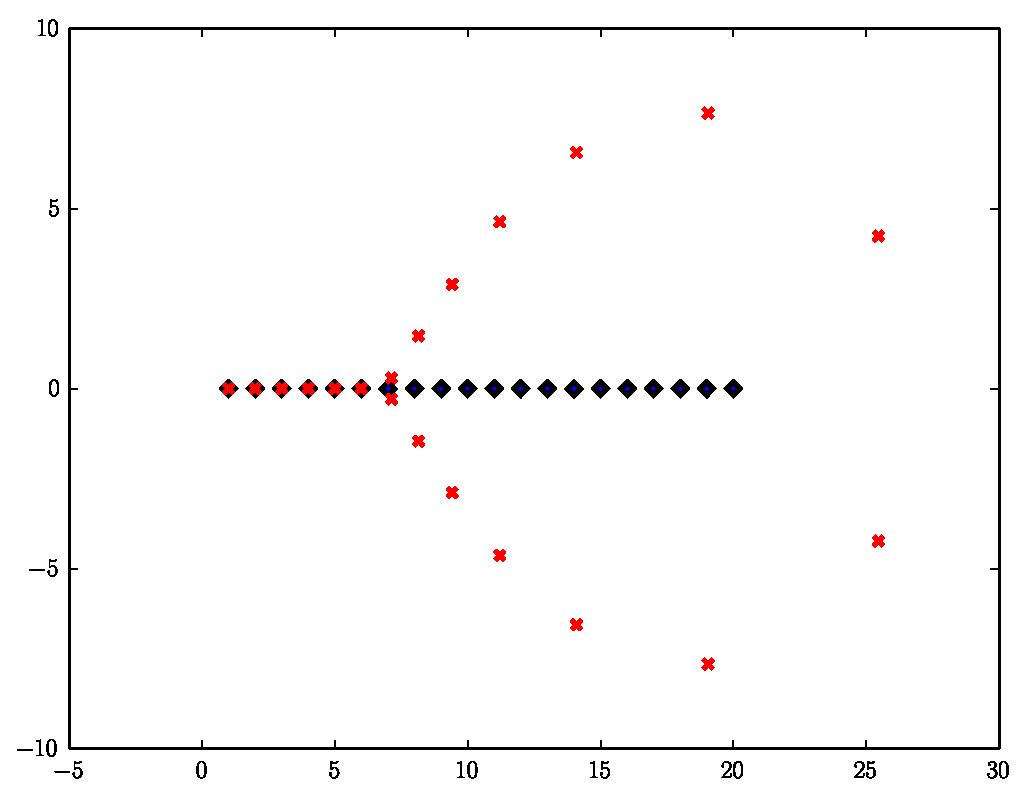
\includegraphics[height=2in]{wilkinsonpolynomial.pdf}
\caption{The blue dots are the roots of w(x). The red dots in the complex plane are roots of a randomly perturbed polynomial with coefficients $\hat{a}_k = a_k(1+r_k)$, where the $r_k$ are normally distributed with mean $0$ and standard deviation $10^{-5}$.}
\label{fig:wilkinsonpolynomial}
\end{figure}

\begin{problem}
Write a function to reproduce Figure \ref{fig:wilkinsonpolynomial}.
Perturb $w(x)$ as described in the caption for this Figure.
Instead of plotting the roots for just one random pertubation of $w(x)$, plot the roots for several random perturbations.

Write another function that, given an array of roots for a polynomial, computes the polynomial object representing the polynomial with the desired roots, then finds the roots of the resulting polynomial and plots them with the original roots.
You may find the \li{numpy.poly} function useful for this.
Be sure you use different colors for the different sets of points.
Using equispaced points at integer values, what does the degree of the polynomial have to be for this computation to return incorrect answers?
\end{problem}

\paragraph{Example 2: Calculating Eigenvalues}

Consider the problem of finding the eigenvectors of a given $n \times n$ matrix $A$. If $A$ is symmetric, then fortunately the eigenvalue problem is well-conditioned. However the problem can be extremely ill-conditioned for non-symmetric matrices, even if $n$ is small. For example, the two matrices 
\[ \left( \begin{array}{cc}
1 & 1000 \\
0 & 1
\end{array} \right)
%
\left( \begin{array}{cc}
1 & 1000 \\
0.001 & 1
\end{array} \right)
\]
have eigenvalues $\{ 1,1\}$ and $\{0,2 \}$ respectively.

\begin{problem}
Let $f:X\rightarrow Y$ be a function that accepts an $n\times n$ matrix $A$ and returns an $n \times 1$ vector of eigenvalues $y$. Write your own function that accepts a matrix $A$ and estimates the condition number $\mathcal{K}$ of $f$ at $A$. Recall that the definition of $\mathcal{K}$ in Equation \ref{def:relativeconditionnumber} includes the limit as $\delta \rightarrow 0$ and the supremum over all possible $\delta x \leq \delta$. To mimic this on a computer, simply take $\delta$ to be very small. Then calculate $\mathantt{k} =  { \frac{|| \delta f||}{||f(x)||} } / { \frac{|| \delta x||}{||x||} } $ a large number of times, taking a random $\delta x$ each time such that $||\delta x|| \leq \delta$. Let $\mathcal{K}$ be the largest of the values $\mathantt{k}$ calculated. (Hint: Let each $\delta x$ be a random normal matrix with mean $0$ and standard deviation $\approx 10^{-4}$.)

Experiment with inputting random symmetric and non-symmetric matrices. Remember that if $A$ is any matrix, then $A'A$ is symmetric. What kinds of condition numbers do you get for symmetric vs. non-symmetric matrices? What kinds of matrices give the biggest condition numbers for the eigenvalue problem?
\end{problem}

\paragraph{Example 3: Condition of a System of Equations}
Consider the system of equations
\[ Ax = b
\] for an $n \times n$ matrix $A$ and $n \times 1$ vectors $x$ and $b$. If we hold $A$ fixed, consider the problem of computing $b$ with respect to small changes in $x$. Alternatively, hold $A$ fixed and consider the problem of computing $x = A^{-1} b$ with respect to small changes in $b$. Finally, we may hold $b$ fixed and consider the problem of computing $x = A^{-1}b$ with respect to small changes in $A$.

It turns out that each of these problems has the \emph{same} relative condition number. This number is 
\[
\mathcal{K} (A) = \|A\|_2 \|A^{-1}\|_2
\]

This is called the \emph{condition number of $A$}.
The condition number of a matrix can be computed using \li{numpy.linalg.cond}.

Notice that the condition number of a matrix cannot be less that $1$.
It is almost always best to work with orthonormal matrices (or operations that can be mathematically represented by orthonormal matrices).
Since orthonormal matrices have a norm of $1$, as do their inverses, these transformations have the best possible condition number.
The low condition number of orthonormal matrices is one of the primary reasons that Householder reflections and Givens rotations are used in so many algorithms.

\section*{Stability of an Algorithm}

The analysis of problem-solving given above assumed that for a given input $\hat{x}$, we could determine the correct output $f(\hat{x})$ exactly. In other words, even if $\hat{x} \neq x$, we assumed that we could calculate $f(\hat{x})$ exactly although it may be different from $f(x)$. 

In practice, our calculation of $f(\hat{x})$ is not always accurate, \emph{even if} the problem $f$ is well-conditioned. Our method of solving the problem may introduce new error. Sometimes the new error we introduce may be very large. 

We define an \emph{algorithm} to be a method of solving a given problem. (The algorithm for solving a problem is different than the problem itself.) If an algorithm introduces large errors while solving a problem, the algorithm is called \emph{unstable}. A \emph{stable} algorithm does not introduce large error while solving a problem.

What could go wrong in an algorithm that would introduce new errors? Usually this happens when the algorithm breaks the problem into sub-problems, and one of these sub-problems is ill-conditioned. For example, the problem of computing the matrix $e^A$ may be well-conditioned for a given $A$, while the problem of computing the eigenvalues and eigenvectors of the same $A$ may be ill-conditioned. If an algorithm for computing $e^A$ relies on the intermediate step of computing the eigenvalues and eigenvectors, new error will be introduced. 

As another example, take the problem of computing the eigenvalues of a matrix $A$. If $A$ is symmetric, the eigenvalue problem is well-conditioned. However, suppose we use an algorithm that first computes the coefficients of the characteristic polynomial, and then finds the roots of that polynomial. Unavoidably, tiny errors will creep in when we compute the coefficients of the characteristic polynomial. Since root-finding is an ill-conditioned problem, these tiny errors will be magnified. This algorithm is unstable.

\begin{warn}
Be careful to not confuse the stability of an algorithm with the conditioning of a problem.
These are two very different things.
A stable algorithm is, roughly speaking, an algorithm that will return a correct result if the problem is well conditioned.
If a problem is poorly conditioned, special algorithmic changes may be necessary to ensure a reasonable degree of accuracy.
\end{warn}

\paragraph{Example 4: A Simple but Unstable Algorithm}
Consider
\[\int_0^1 x^n e^{x - 1} dx\]
It is easily seen that this integral is always positive and always less than $1$.
It can be shown that, when $n > 1$, the value for this integral is always equal to
\[\left(-1\right)^{n} !n + \left(-1\right)^{n + 1} \frac{n!}{e}\]
where $!n$ is a combinatorial function called a derangement (it is equal to the number of permutations of a set that change the position of each element).
$!n$ is given by the recurrence relation $\left(n - 1\right)\left(!\left(n - 1\right) + !\left(n - 2\right)\right)$ and is defined to have the initial values $!0 = 1$ and $!1 = 0$.
There is a similar recurrence relation for the factorial function.
Given these recurrence relations, we can compute the value for this integral as using the following blocks of code:
\begin{lstlisting}
import numpy as np
def derangement(n):
    d0, d1 = 1, 0
    for i in xrange(1, n):
        d0, d1 = d1, i * (d0 + d1)
    return d1
def factorial(n):
    d0, d1 = 1, 1
    for i in xrange(1, n):
        d0, d1 = d1, i * (d0 + d1)
    return d1
def integral(n):
    return (-1)**n * derangement(n) + (-1)**(n-1) * factorial(n) / np.e
\end{lstlisting}
Unfortunately, since we are taking the difference of large floating point numbers that are very close to one another, this algorithm only gives correct values for the first few integrals.
The output is shown in Table \ref{table:unstable_computation}.

\begin{table}
\centering
\begin{tabular}{|l|l|l|}
\hline
Integrand & Computed Value & Actual Value \\
\hline
$x^{1}e^{x}$: & $0.367879441171$ & $0.367879441171$ \\
$x^{5}e^{x}$: & $0.145532940573$ & $0.145532940573$ \\
$x^{10}e^{x}$: & $0.0838770701084$ & $0.0838770701034$ \\
$x^{15}e^{x}$: & $0.0590209960938$ & $0.0590175408793$ \\
$x^{20}e^{x}$: & $0.0$ & $0.0455448840758$ \\
$x^{25}e^{x}$: & $1073741824.0$ & $0.0370862144237$ \\
$x^{30}e^{x}$: & $-1.80143985095 \cdot 10^{16}$ & $0.0312796739322$ \\
$x^{35}e^{x}$: & $6.04462909807 \cdot 10^{23}$ & $0.0270462894091$ \\
$x^{40}e^{x}$: & $0.0$ & $0.023822728669$ \\
$x^{45}e^{x}$: & $0.0$ & $0.0212860390856$ \\
$x^{50}e^{x}$: & $1.46150163733 \cdot 10^{48}$ & $0.0192377544343$ \\
\hline
\end{tabular}
\caption{Inaccuracy of values computed using an unstable algorithm.}
\label{table:unstable_computation}
\end{table}

The algorithms that we have studied to solve linear systems have different levels of stability.
LU decomposition (with pivoting) is usually good enough, but there are some pathological examples of matrices that cause it to break down.
QR decompositoin (with pivoting) is generally considered to be a better option than the LU decomposition.
Solving a linear system using the SVD is even more stable than the QR decomposition.
(Pivoting is a modification that is commonly made to the LU decomposition and QR decompositoin algorithms we have discussed in earlier labs to make them more stable.)
Unfortunately, in this case, the algorithms that more stable are also slower.
The LU decomposition is used by \li{scipy.linalg.solve}.
The SVD is used by \li{scipy.linalg.lstsq}.
Here is some code that uses the QR decomposition of a matrix $A$ to solve the linear system $A x = b$ for $x$.
It uses a lower-level function included in scipy to perform the back substitution required to solve this system.
\begin{lstlisting}
from scipy import linalg as la
from scipy.linalg.flapack import dtrtrs
def qr_solve(A, b):
    Q, R = la.qr(A)
    return dtrtrs(R.T, Q.T.dot(b), lower=1, trans=1)[0]
\end{lstlisting}
A solution using a pivoted QR decomposition would be better, but this will be good enough for demonstration purposes.

The following are routines that generate matrices designed to show the relative benefits of each of these algorithms.
\begin{lstlisting}
from numpy.random import rand

def bad_arr_1(n):
    """ Construct a specific pathological example
    that breaks LU decomposition. These examples
    are very rare, but they do exist.
    Strictly speaking, the condition number
    for this matrix isn't terribly bad. """
    A = - np.ones((n, n))
    A[:,:-1] = np.tril(A[:,:-1])
    np.fill_diagonal(A, 1)
    A[:,-1] = 1
    return A

def bad_arr_2(n, peturbation = 1E-8):
    """ Construct another matrix that is nearly singular
    by computing A.dot(A.T) for a matrix A that is
    not square and then adding some small changes
    so it is not exactly singular. """
    A = rand(n, n // 2)
    return A.dot(A.T) + peturbation * rand(n, n)
\end{lstlisting}

\begin{problem}
For each of the array creation routines above, plot the error $\norm{\text{solve}\left(A, A b\right) - b}$ of each of the methods mentioned above for solving a linear system.
Use a log-scaled $y$-axis.
What do you observe?
\end{problem}

%\subsection*{Stable vs. Backward Stable Algorithms}

%\subsection*{Table}
%
%\begin{table}[h]
%\begin{tabular}{|l|l|l|}
%\hline \textbf{Well-Conditioned} & \textbf{Ill-Conditioned} & \textbf{Systems of Equations} \\
%{\parbox{0.3\textwidth}{\raggedleft
%            \begin{itemize}[leftmargin=*]
%                \item finding eigenvalues of a symmetric (or normal) matrix 
%                \item calculating $e^x$ for relatively small values of $x$ 
%                \item calculating $\ln(x)$ for $x$ not close to $1$
%            \end{itemize} }}           &  
%             
%{\parbox{0.3\textwidth}{\raggedleft
%            \begin{itemize}[leftmargin=*]
%                \item calculating $x_1 - x_2$ when $x_1 \approx x_2$ 
%                \item computing roots of a polynomial, given the coefficients
%                \item computing eigenvalues of a non-symmetric matrix
%            \end{itemize} }}              &   
%            
%{\parbox{0.3\textwidth}{
%            \begin{itemize}[leftmargin=*]
%                 \item relative condition number is \[ \mathcal{K} = ||A|| ||A^{-1}|| \]
%            \end{itemize} }}   \\ \hline                      
%\end{tabular}
%\end{table}
%
%
%\begin{table}[h]
%\begin{tabular}{|l|l|}
%\hline \textbf{Stable} & \textbf{Unstable} \\
%{\parbox{0.45\textwidth}{\raggedleft
%            \begin{itemize}[leftmargin=*]
%                \item finding eigenvalues of a symmetric (or normal) matrix 
%                \item calculating $e^x$ for relatively small values of $x$ 
%                \item calculating $\ln(x)$ for $x$ not close to $1$
%            \end{itemize} }}           &  
%             
%{\parbox{0.45\textwidth}{\raggedleft
%            \begin{itemize}[leftmargin=*]
%                \item calculating $x_1 - x_2$ when $x_1 \approx x_2$ 
%                \item computing roots of a polynomial, given the coefficients
%                \item computing eigenvalues of a non-symmetric matrix
%            \end{itemize} }}    \\ \hline                      
%\end{tabular}
%\end{table}
%
